\documentclass{beamer}
\usetheme{CambridgeUS}

\usepackage{graphicx}
\usepackage{subcaption}
\usepackage{natbib}
\usepackage{booktabs}

\DeclareMathOperator*{\argmin}{argmin}

\title[node2vec]{node2vec: Embedding of Networks}
\author{David McDonald}
%\institute{University of Birmingham, \\ Birmingham, UK \\ B15 2TT}
\date{21st August 2017}

\begin{document}
	
	\begin{frame}
		\titlepage
	\end{frame}

	\begin{frame}{Some Context: Why embed networks?}
		\begin{itemize}
			\item Visualisation
			\item feature extraction
			\item Similar nodes should be embedded close together
			\item Bijection
		\end{itemize}
	\end{frame}
	
	\begin{frame}{Introduction}
		For our model we are taking inspiration from Natural Language Processing (NLP):
		
		\begin{itemize}
			\item How can we learn vector representations of words?
			\item `similar' words should be mapped close together
			\item how do can a machine learn these semantics?
		\end{itemize}
		 
	\end{frame}
	
	\begin{frame}[allowframebreaks]{Skipgram Model}
		\begin{itemize}
			\item We are going to train a neural network with a single layer to perform a task
			\item But we are not going to use the neural network for the task it was trained on!
			\item We will use the weights of the hidden layer -- which will be the word representations that we are looking for
		\end{itemize}
		
		\pagebreak
		
		We have seen this technique before
		
		In an autoencoder:
		
		
		\pagebreak
		
		What is the task that we are training on?
		
		Given a sentence an input word, our network will tell us the how likely it is that we see the words in the sentence close to our input word
		
		\begin{itemize}
			\item Window size
		\end{itemize}
		
		\begin{figure}
			\centering
			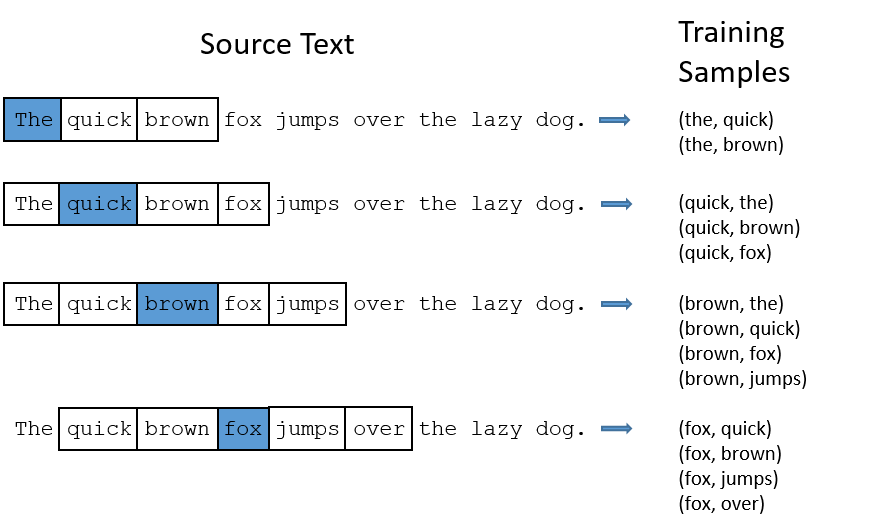
\includegraphics[width=\textwidth]{presentation_5_figures/training_data}
		\end{figure}
		
	\end{frame}
	
	\begin{frame}{Training}
		Our model learns probabilities of the form
		\begin{align*}
		p(y | x)
		\end{align*}
		
		for example, given (the, quick) as a training sample, we aim to maximise
		
		\begin{align*}
		p(\text{quick} | \text{the})
		\end{align*}
		
		and minimise
		
		\begin{align*}
		p(\text{*anything else*} | \text{the})
		\end{align*}
	\end{frame}
	
	\begin{frame}[allowframebreaks]{The Model}
		Lets say out vocabulary is 10000 words and we want to learn a 300 dimensional embedding:
		\begin{itemize}
			\item Input: one hot vector of length 10000
			\item Hidden: 300 linear neurons
			\item Output: also a vector of length 10000
		\end{itemize}
		
		\pagebreak
%		
		\begin{figure}
			\centering
			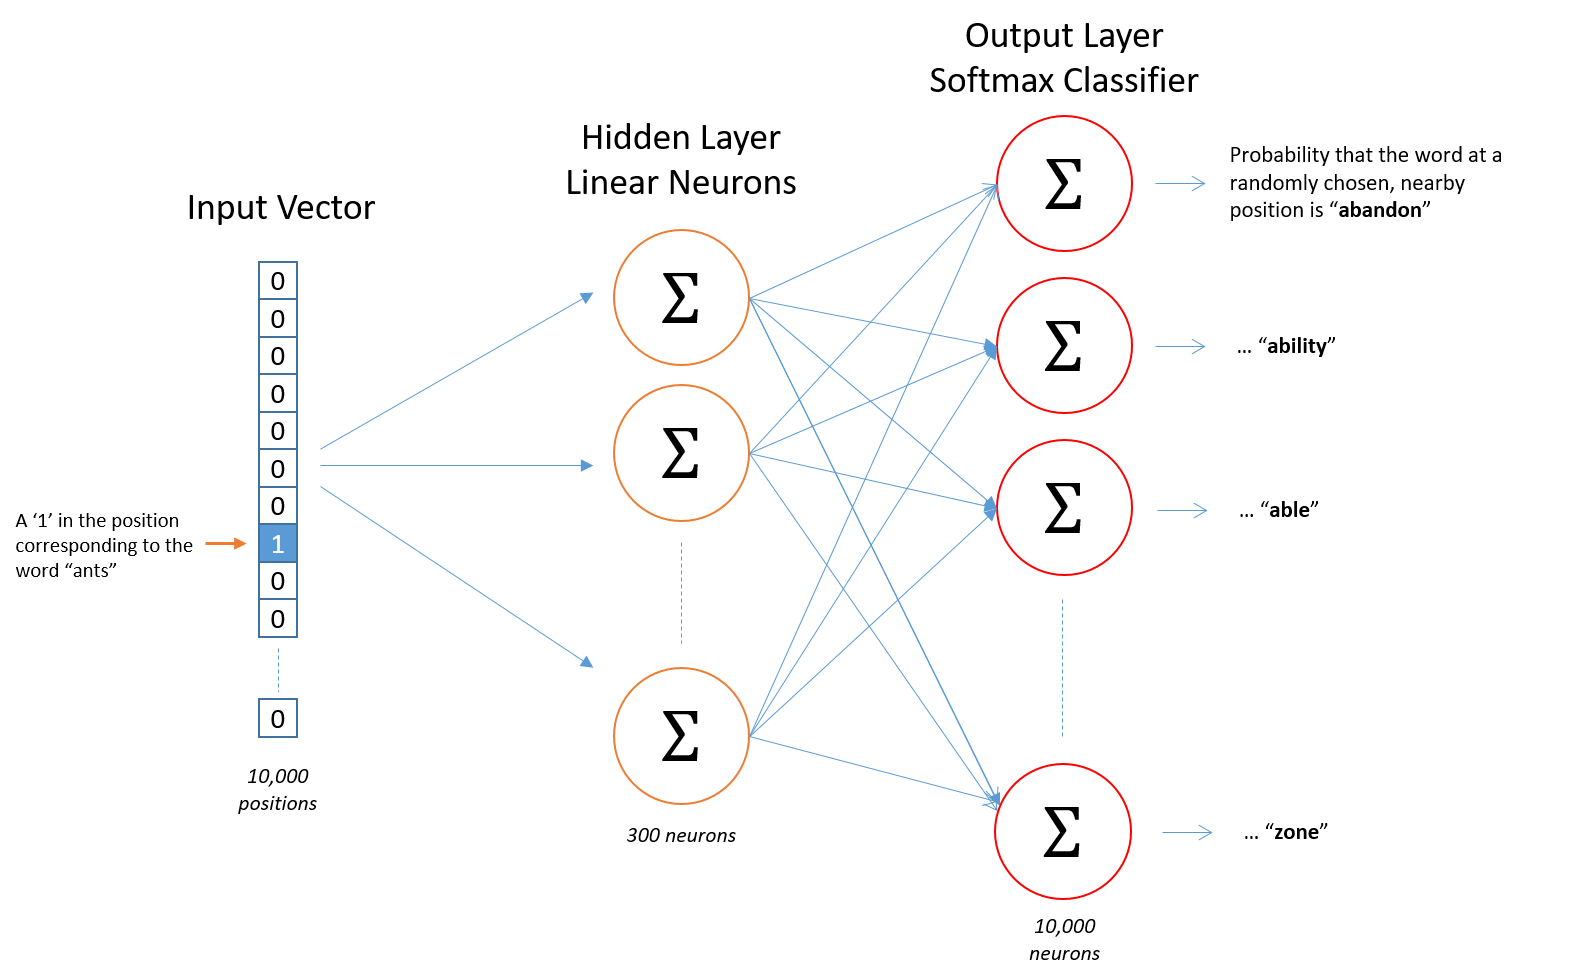
\includegraphics[scale=0.4]{presentation_5_figures/skip_gram_net_arch}
		\end{figure}
		
	\end{frame}
		
	\begin{frame}[allowframebreaks]{The Hidden Layer}
		
		Toy example: vocabulary size of 5, embedding dimension 30
		
		\begin{figure}
			\centering
			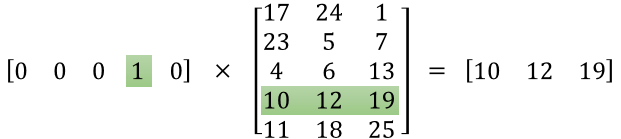
\includegraphics[width=\textwidth]{presentation_5_figures/matrix_mult_w_one_hot}
		\end{figure}
		
		The rows of the hidden weight matrix become our word representations!
		
		We just toss the output layer after we have finished training.
		
		\pagebreak
		
		Back to 10000 words and 300 dimensions:

		\begin{figure}
			\centering
			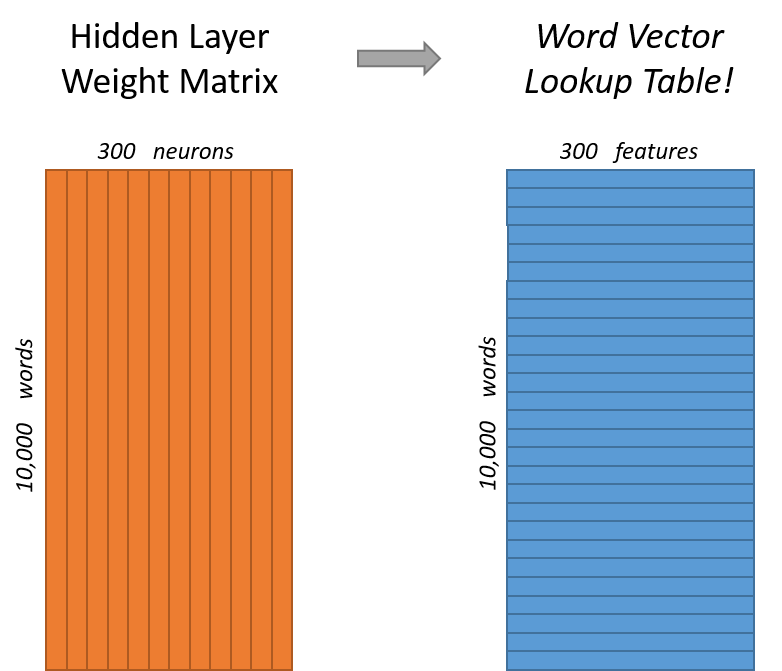
\includegraphics[scale=0.5]{presentation_5_figures/word2vec_weight_matrix_lookup_table}
		\end{figure}

		
	\end{frame}
	
	\begin{frame}[allowframebreaks]{The Output Layer}
		Softmax regression:
		\begin{align*}
		\text{Softmax}(h W_{,i}^{out}) = \frac{\exp(h W_{,i}^{out}))}{\sum_{j}\exp(h W_{,j}^{out}))}
		\end{align*}
		\begin{itemize}
			\item Each neuron (one for each word in the vocabulary) will output a number between 0 and 1
			\item All outputs will sum to 1
		\end{itemize}
		The columns in $W^{out}$ become `neighbour' representation of the words.
		When the hidden representation of our input word ($h$) is similar to $W_{,i}$ then $hW_{,i}$ is large
	\end{frame}
	
	\begin{frame}{Recap}
		\begin{itemize}
			\item We train by feeding the model pairs of input/target words determined by `context window'
			\item We use one hot representations as input/targets
			\item We train using Softmax to maximise probability of observing target word, given the input word
		\end{itemize}
	\end{frame}
	
	\begin{frame}{Some Problems}
		
		\begin{itemize}
			\item Our model has a lot of parameters to estimate: $\approx$10000 x 300 + 300 x 10000
			\item Back propagation with Softmax requires knowledge of all the outputs
			\item Millions of training examples
		\end{itemize}
		
		All of this leads to very slow training!
		
		3 adaptions to speed up training (and obtain better results!)
		
		
	\end{frame}
	
	\begin{frame}{Phrases}
		\begin{itemize}
			\item scan through text and look for words that frequently appear together
			\item for example, `New' and `York'
			\item and add these 'phrases' to the vocabulary
		\end{itemize}
	\end{frame}
	
	\begin{frame}{Subsampling}
		\begin{figure}
			\centering
			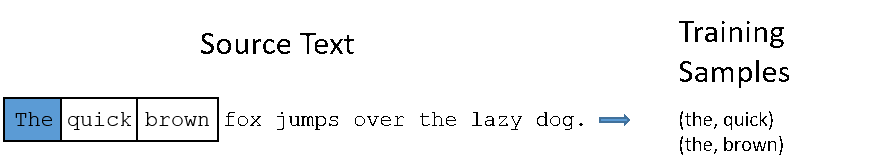
\includegraphics[width=\textwidth]{presentation_5_figures/training_data_cut}
		\end{figure}
		\begin{itemize}
			\item We would like to cut frequent words from our text
			\item For example the word `the' does not tell us very much about the word `brown'
			\item the probability of deletion is proportional to frequency
			\item if we cut a specific instance of the word `the', then it will not appear in the contexts of any nearby words
		\end{itemize}
	
	\end{frame}
	

	
	\begin{frame}[allowframebreaks]{Negative Sampling}
		
		\begin{itemize}
			\item Each training sample will adjust \textbf{all} the weights in the network a tiny bit
			\item with negative sampling, we only select a small number of negative samples (say, 5) to adjust the weights for
			\item negative samples are words that we want the network to output a 0 for
			\item we also want to update the weights of the positive example
			
			\pagebreak
			
			\begin{figure}
				\centering
				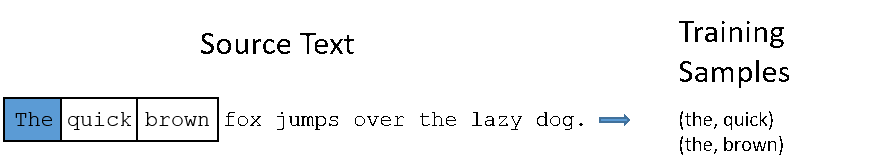
\includegraphics[width=\textwidth]{presentation_5_figures/training_data_cut}
			\end{figure}
			
			For the training pair (the, quick), we would adjust the weights for 
			\begin{itemize}
				\item quick (our positive sample)
				\item 5 randomly chosen negative samples (that never appear in the context of the input word `the')
			\end{itemize}

			Negative samples are also chosen according to frequency.
		\end{itemize}
		
		
	\end{frame}
	
	\begin{frame}[allowframebreaks]{node2vec}
		
		So how is this relevant at all to network embedding?
		
		\pagebreak
		
		We can use random walks to generate the `neighbourhood' of a node and use that as its `context'.
		
	\end{frame}
	
	\begin{frame}[allowframebreaks]{Generating the Context of a Node}

		Given a source node $u$, we define a random walk of length $l$ as a sequence $c_0, ..., c_l$ defined by the following probability distribution:
		
		\begin{align*}
		P(c_i = x | c_{i-1} = v, c_{i-2}=t) = 
		\begin{cases}
		\frac{\alpha_{tx} w_{xv}}{Z} &\text{if } (x, v) \in E, \\
		0, &\text{otherwise.}
		\end{cases}
		\end{align*}
		
		\begin{columns}
			\begin{column}{0.45\textwidth}

				with 
				\begin{align*}
				\alpha_{tx} = 
				\begin{cases}
				\frac{1}{p} & \text{if } d(t, x) = 0,\\
				1 & \text{if } d(t, x) = 1,\\
				\frac{1}{q} & \text{if } d(t, x) = 2.
				\end{cases}
				\end{align*}
			\end{column}
			
			\begin{column}{0.45\textwidth}
				\begin{figure}
					\centering
					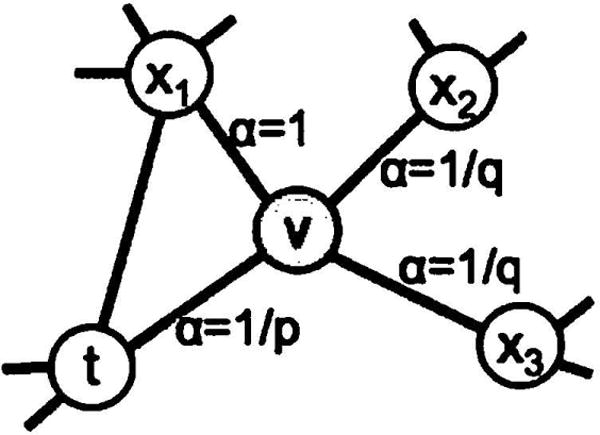
\includegraphics[width=\textwidth]{presentation_5_figures/random_walk}
				\end{figure}
			\end{column}
		\end{columns}
		
		\pagebreak
		
		\begin{itemize}
			\item $l$ is the context size
			\item $p$ is the \textit{return parameter}
			\begin{itemize}
				\item setting it to a high value reduces the chance of backtracking
				\item a low setting keeps the search close (local) (BFS)
			\end{itemize}
			\item $q$ is the \textit{in-out parameter}
			\begin{itemize}
				\item $q>1:$ biases towards nodes close to $t$
				\item $q<1:$ biases towards nodes further away (DFS)
			\end{itemize}
			\item Walks are second order Markovian
		\end{itemize}
		
		
	\end{frame}
	
	\begin{frame}{Example on Les Miserables Network}
		\begin{figure}
			\centering
			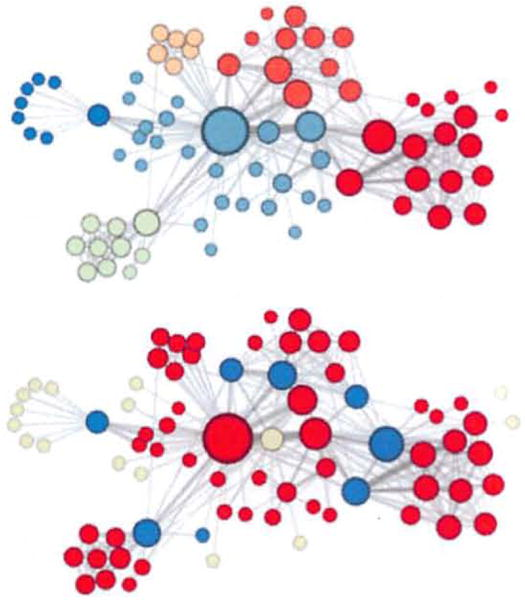
\includegraphics[scale=0.7]{presentation_5_figures/nihms825755f3}
		\end{figure}
	\end{frame}
	
	\begin{frame}{Extensions}
		\begin{itemize}
			\item Multi-layer networks
			\item Node attributes
			\item Hyperbolic space
		\end{itemize}
	\end{frame}
	
	\begin{frame}{A recommended blog}
		\url{http://mccormickml.com/2016/04/19/word2vec-tutorial-the-skip-gram-model/}
	\end{frame}

\end{document}